\section{Auswertung}
\label{sec:Auswertung}

\subsection{Auftragen der Messwerte}
Zunächst werden die Grenzspannungen $U_G$ der jeweiligen Spektrallinien bestimmt.
Dafür werden in \autoref{fig:spek1} bis \autoref{fig:spek5} die Gegenspannungen gegen die Wurzel des Stroms aufgetragen.
Die jeweiligen Messwerte dazu sind in den Tabellen \ref{tab:spek1} - \ref{tab:spek5} zu finden.
Die Grenzspannung wird durch den Ansatz
\begin{equation*}
  U_G = - \frac{b}{a}
\end{equation*}
berechnet, da es sich um eine Gerade handelt.
Für die Ausgleichsgerade ergeben sich die in \autoref{tab:paramgeraden} errechneten Werte.

\begin{table}
  \centering
  \caption{Werte der Parameter der Regressionsgeraden}
  \label{tab:paramgeraden}
  \begin{tabular}{ |p{3cm}||p{3cm}|p{3cm}|p{3cm}|  }
    \hline
    Farbe & $a$ & $b$ & $U_\text{G}$ \\
    \hline
    Ultraviolett   &  -0.832 ± 0.029   & 1.188 ± 0.021 &   1.430 ± 0.060\\
    Violett &   -2.491 ± 0.088  & 3.078 ± 0.059   & 1.24 ± 0.05\\
    Grün & -3.949 ± 0.164 & 2.711 ± 0.063 & 0.687 ± 0.033\\
    Gelb    & -2.856 ± 0.120 & 1.599 ± 0.039 & 0.560 ± 0.039\\
    Rot &  -0.531 ± 0.033  & 0.302 ± 0.010 & 0.570 ± 0.040\\
    \hline
   \end{tabular}
\end{table}

\begin{table}
  \centering
  \caption{Messwerte der ultravioletten Linie.}
  \label{tab:spek1}
  \begin{tabular}{c c}
    \toprule
    U / V & I / 10\textasciicircum -9 A \\
    \midrule
    1.283 &         0,0 \\
      1,2 &        0,04 \\
      1,1 &       0,075 \\
      1,0 &       0,145 \\
      0,9 &         0,2 \\
      0,8 &       0,298 \\
      0,7 &       0,415 \\
      0,6 &       0,540 \\
      0,5 &       0,660 \\
      0,4 &       0,780 \\
      0,3 &       0,920 \\
      0,2 &         1,0 \\
      0,1 &         1,2 \\
     0,05 &         1,2 \\
     0,00 &         1,3 \\
    \bottomrule
  \end{tabular}
\end{table}

\begin{table} 
  \centering
  \caption{Messwerte der violetten Linie.}
  \label{tab:spek2}
  \begin{tabular}{c c}
    \toprule
    U / V & I / 10\textasciicircum -9 A \\
    \midrule
    1,152 &         0,0 \\
      1,1 &        0,08 \\
      1,0 &        0,34 \\
      0,9 &        0,72 \\
      0,8 &         1,2 \\
      0,7 &         2,0 \\
      0,6 &         2,9 \\
      0,5 &         4,0 \\
      0,4 &         5,0 \\
      0,3 &         5,9 \\
      0,2 &         6,8 \\
      0,1 &         7,0 \\
     0,05 &         8,2 \\
     0,00 &         8,7 \\
    \bottomrule
    \end{tabular}
\end{table}

\begin{table}
  \centering
  \caption{Messwerte der grünen Linie.}
  \label{tab:spek3}
  \begin{tabular}{c c}
    \toprule
    U / V & I / nA \\
    \midrule
    0,645 &    0,0 \\
      0,6 &   0,12 \\
     0,55 &  0,295 \\
     0,50 &   0,56 \\
     0,45 &   0,62 \\
     0,40 &    1,4 \\
     0,35 &    2,0 \\
      0,3 &    2,8 \\
     0,25 &    3,5 \\
      0,2 &    4,2 \\
     0,15 &    4,8 \\
      0,1 &    5,3 \\
     0,05 &    5,8 \\
      0,0 &    6,2 \\
    \bottomrule
    \end{tabular}
\end{table}

\begin{table}
  \centering
  \caption{Messwerte der gelben Linie.}
  \label{tab:spek4}
  \begin{tabular}{c c c c}
    \toprule
    U / V & I / nA & U / V.1 & U / nA \\
    \midrule
     0,52 &    0,0 &   -0,05 &    2,4 \\
      0,5 &   0,02 &    -0,1 &    2,6 \\
     0,45 &    0,1 &    -0,5 &    3,8 \\
      0,4 &   0,22 &    -1,0 &    5,4 \\
     0,35 &    0,4 &   - 1,5 &    6,4 \\
      0,3 &   0,63 &    -2,0 &    7,6 \\
     0,25 &   0,96 &    -3,0 &   10,0 \\
      0,2 &    1,2 &    -4,0 &   12,0 \\
     0,15 &    1,5 &    -6,0 &   12,0 \\
      0,1 &    1,7 &   -10,0 &   17,0 \\
     0,05 &    2,0 &   -14,0 &   20,0 \\
      0,0 &    2,2 &   -18,0 &   20,0 \\
      NaN &    NaN &    19,0 &   21,0 \\
    \bottomrule
  \end{tabular}
\end{table}

\begin{table}
  \centering
  \caption{Messwerte der roten Linie.}
  \label{tab:spek5}
  \begin{tabular}{c c}
    \toprule
    U / V & I / nA \\
    \midrule
      0,5 &    0,0 \\
     0,45 &  0,005 \\
      0,4 & 0,0075 \\
     0,35 &   0,02 \\
      0,3 &  0,021 \\
     0,25 &  0,035 \\
      0,2 &   0,04 \\
     0,15 &   0,05 \\
      0,1 &   0,06 \\
     0,05 &  0,075 \\
     0,00 &   0,08 \\
    \bottomrule
    \end{tabular}
\end{table}

\begin{figure}
  \center
  \caption{Regressionsgerade der ultravioletten Linie.}\label{fig:spek1}
  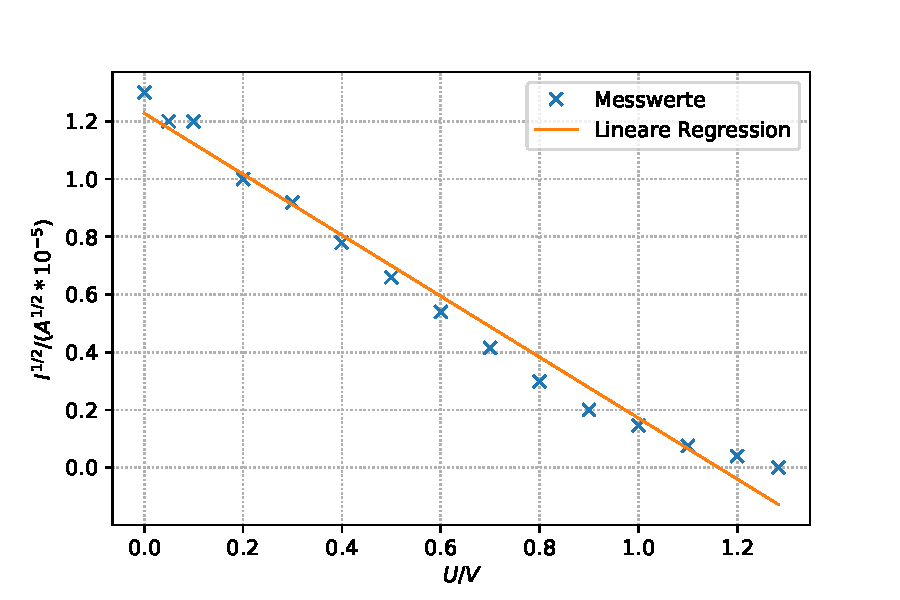
\includegraphics[width=0.8\linewidth]{pictures/spek1.pdf}
\end{figure}

\begin{figure}
  \center
  \caption{Regressionsgerade der violetten Linie.}\label{fig:spek2}
  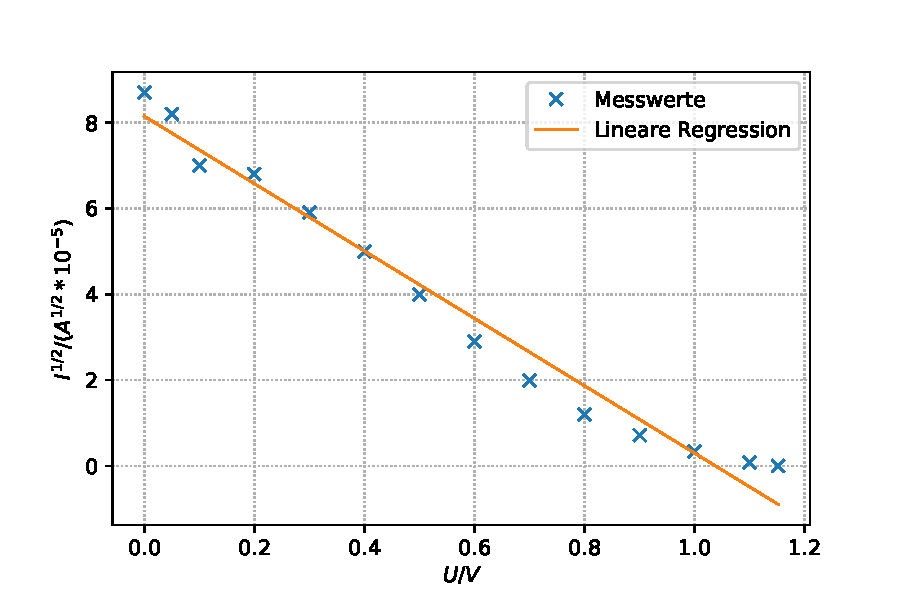
\includegraphics[width=0.8\linewidth]{pictures/spek2.pdf}
\end{figure}

\begin{figure}
  \center
  \caption{Regressionsgerade der grünen Linie.}\label{fig:spek3}
  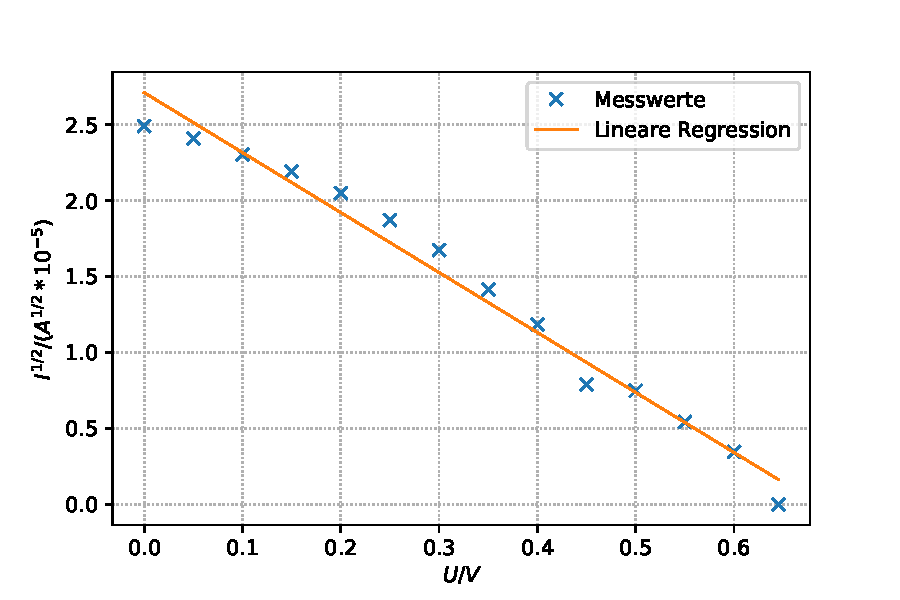
\includegraphics[width=0.8\linewidth]{pictures/spek3.pdf}
\end{figure}

\begin{figure}
  \center
  \caption{Regressionsgerade der gelben Linie.}\label{fig:spek4}
  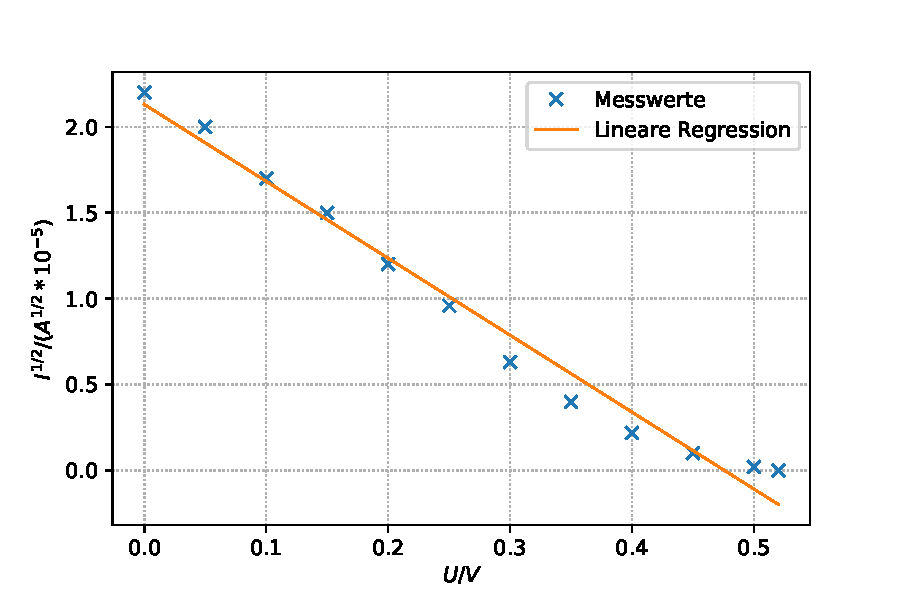
\includegraphics[width=0.8\linewidth]{pictures/spek4.pdf}
\end{figure}

\begin{figure}
  \center
  \caption{Regressionsgerade der roten Linie.}\label{fig:spek5}
  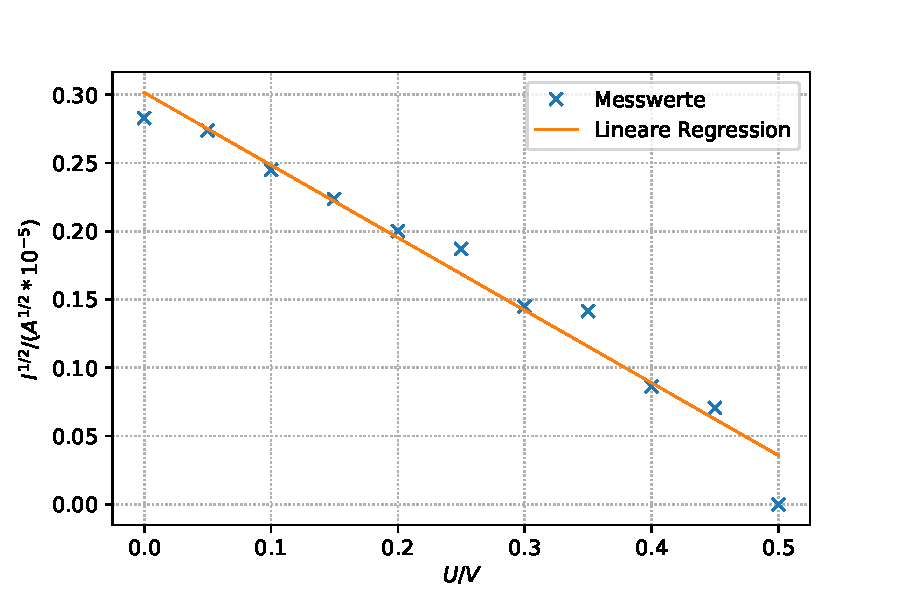
\includegraphics[width=0.8\linewidth]{pictures/spek5.pdf}
\end{figure}


\subsection[Ermittlung von dem Verhältnis h/e und der Austrittsarbeit]{Ermittlung von dem Verhältnis $h / e_0$ und der Austrittsarbeit $A_k$}
% Weil hyperref wegen math meckert: https://tex.stackexchange.com/questions/5314/equations-in-section-heading-title
Nun wird in \autoref{fig:austritt} die Frequenz $\nu$ gegen die Grenzspannung auf der y-Achse aufgetragen.
Die Frequenz berechnet sich durch
\begin{equation}
  \nu = \frac{c}{\lambda}.
\end{equation}
c ist dabei die Lichtgeschwindigkeit und \lambda ist die Wellenlänge.
Die Wellenlängen sind auf dem Praktikumsblatt \cite{v500} zu finden.
%Die Daten für die rote Linie wurde aus einer anderen Seite genommen.

\begin{table}
  \centering
  \caption{Messwerte zur Bestimmung der Austrittsarbeit, sowie des Verhältnisses $\frac{h}{e_0}$.}
  \label{tab:austritt}
  \begin{tabular}{c c c}
    \toprule
    $U_G$ / V & $\lambda / 10^{-9}$ & $\nu / 10^{12} \unit\hertz$ \\
    \midrule
    1.430 & 365 & 821.9\\
    1.24 & 436 & 983.6\\
    0.687 & 546 & 549.4\\
    0.560 & 579 & 519.9\\
    0.570 & 644 & 465.8\\ % Quelle https://www.praktikumphysik.uni-hannover.de/fileadmin/praktikumphysik/Versuche/HF/D-Optik/D08_HF.pdf
    \bottomrule
  \end{tabular}
\end{table}

\begin{figure}
  \center
  \caption{Regressionsgerade zur Bestimmung der Austrittsarbeit.}\label{fig:austritt}
  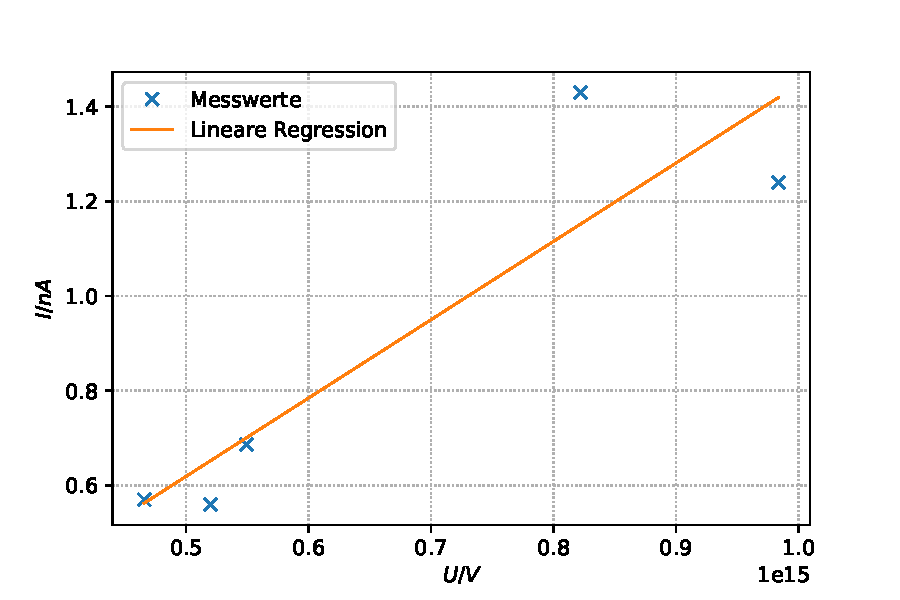
\includegraphics[width=0.8\linewidth]{pictures/austritt.pdf}
\end{figure}

Für die Regressionsgerade ergeben sich die Werte

\begin{align}
  a = \frac{h}{e_0} &= (1.65 ± 0.44) \cdot 10^{-15} \unit{\eV} \\
  &\text{und} \\
  |b| = A_K &= (0.21 ±  0.31) \unit{\eV}.
\end{align}

\subsection{Photostrom in Abhängigkeit der angelegten Spannung am Beispiel der gelben Linie}
\begin{figure}
  \center
  \caption{Messdaten des Photostromes der gelben Linie.}\label{fig:spek4s}
  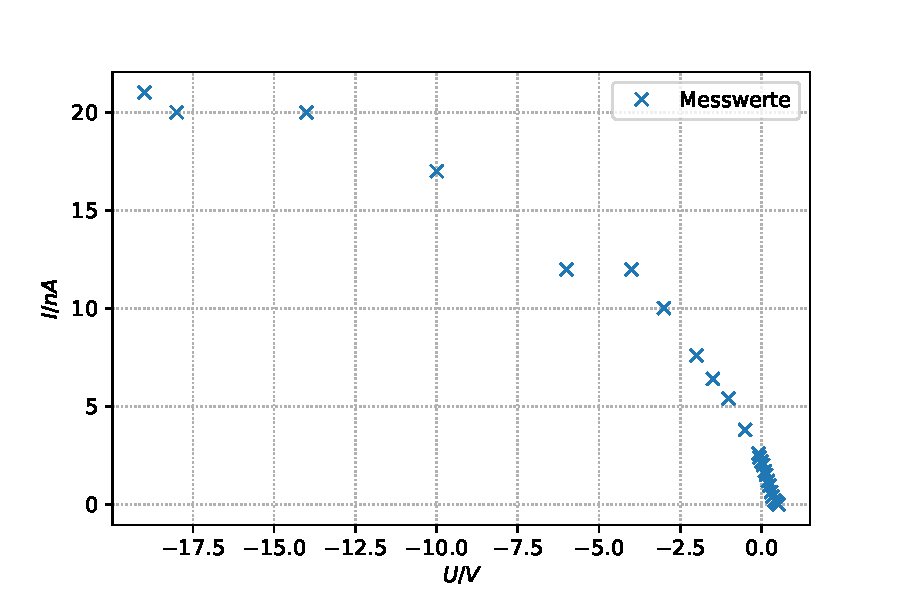
\includegraphics[width=0.8\linewidth]{pictures/spek4s.pdf}
\end{figure}

%Da während des Versuches die Aufnahme der Werte abgebrochen wurde, sobald der Fotostrom null wurde,
%wurde in \autoref{fig:spek4s} der Plot aus anschaulichen Gründen um einige Nullen erweitert.
Die Messwerte sind in \autoref{tab:spek4} und in \autoref{fig:spek4s} dargestellt, wobei die negativen Werte einer Beschleunigungsspannung gleich sind.